\section{Evaluation}
\label{sec:eval}

With the advancement of Large Language Models, the performance of models in complex document processing and RAG tasks has become a central focus of research. This section reviews evaluation benchmarks spanning visual document understanding, document QA, and real-world image-text interaction scenarios.

\subsection{Visual Document Understanding and Basic QA Evaluation}

Document Question Answering (DocQA) research focuses on whether models can correctly understand text, layout, and visual cues from single-page or small-scale documents.

\subsubsection{Single-Page Document Understanding}

DocVQA \cite{docvqa2020} was among the earliest benchmarks to systematically propose ``question answering on document images,'' emphasizing fact localization through understanding text, layout, and visual cues in single-page documents. Document Collection VQA \cite{doccollectionvqa2021} first placed questions in document collection scenarios, requiring models to locate answers across multiple documents. InfographicVQA \cite{infographicvqa2021} focused on infographic QA to evaluate understanding and reasoning in mixed scenarios of complex layouts, charts, and text.

Scientific and information-seeking benchmarks included A Dataset of Information-Seeking Questions and Answers Anchored in Research Papers \cite{infoseekqa2021}, focusing on question types readers actually ask. DUE \cite{due2021} proposed a comprehensive end-to-end document understanding benchmark where models start from raw documents and complete downstream tasks.

\subsubsection{Cross-Page and Long-Document Understanding}

Research shifted from ``understanding one page'' to ``cross-page understanding and localization.'' Hierarchical Multimodal Transformers for Multi-Page DocVQA \cite{tito2023hierarchicalmultimodaltransformersmultipage} first systematically handled multi-page documents through hierarchical structural modeling. VRDU \cite{vrdu2023} proposed a benchmark specifically for complex business document information extraction. Test-Time Adaptation for Visual Document Understanding \cite{tta-vdu2023} enabled model adaptation at test time.

Datasets with ``locating evidence from many pages'' problem settings emerged. PDFVQA \cite{pdfvqa2023} introduced real PDF documents where questions require locating key information among many pages. SlideVQA \cite{slidevqa2023} studied understanding and reasoning across multiple slide pages. DUDE \cite{dude2023} and DLUE \cite{dlue2023} provided comprehensive evaluation frameworks for visually rich and long complex-structured documents.

Specialized benchmarks addressed particular challenges. KNVQA \cite{knvqa2023} assessed ``factuality'' and knowledge reasoning abilities of Large Vision-Language Models. Privacy-Aware Document VQA \cite{privacydocvqa2023} studied automatic QA under Federated Learning and Differential Privacy constraints. PDFTriage \cite{saad2024pdftriage} evaluated QA capabilities in ``whole book / ultra-long context'' scenarios, emphasizing document structure roles in retrieval and answering.

\begin{figure*}[t]
\centering
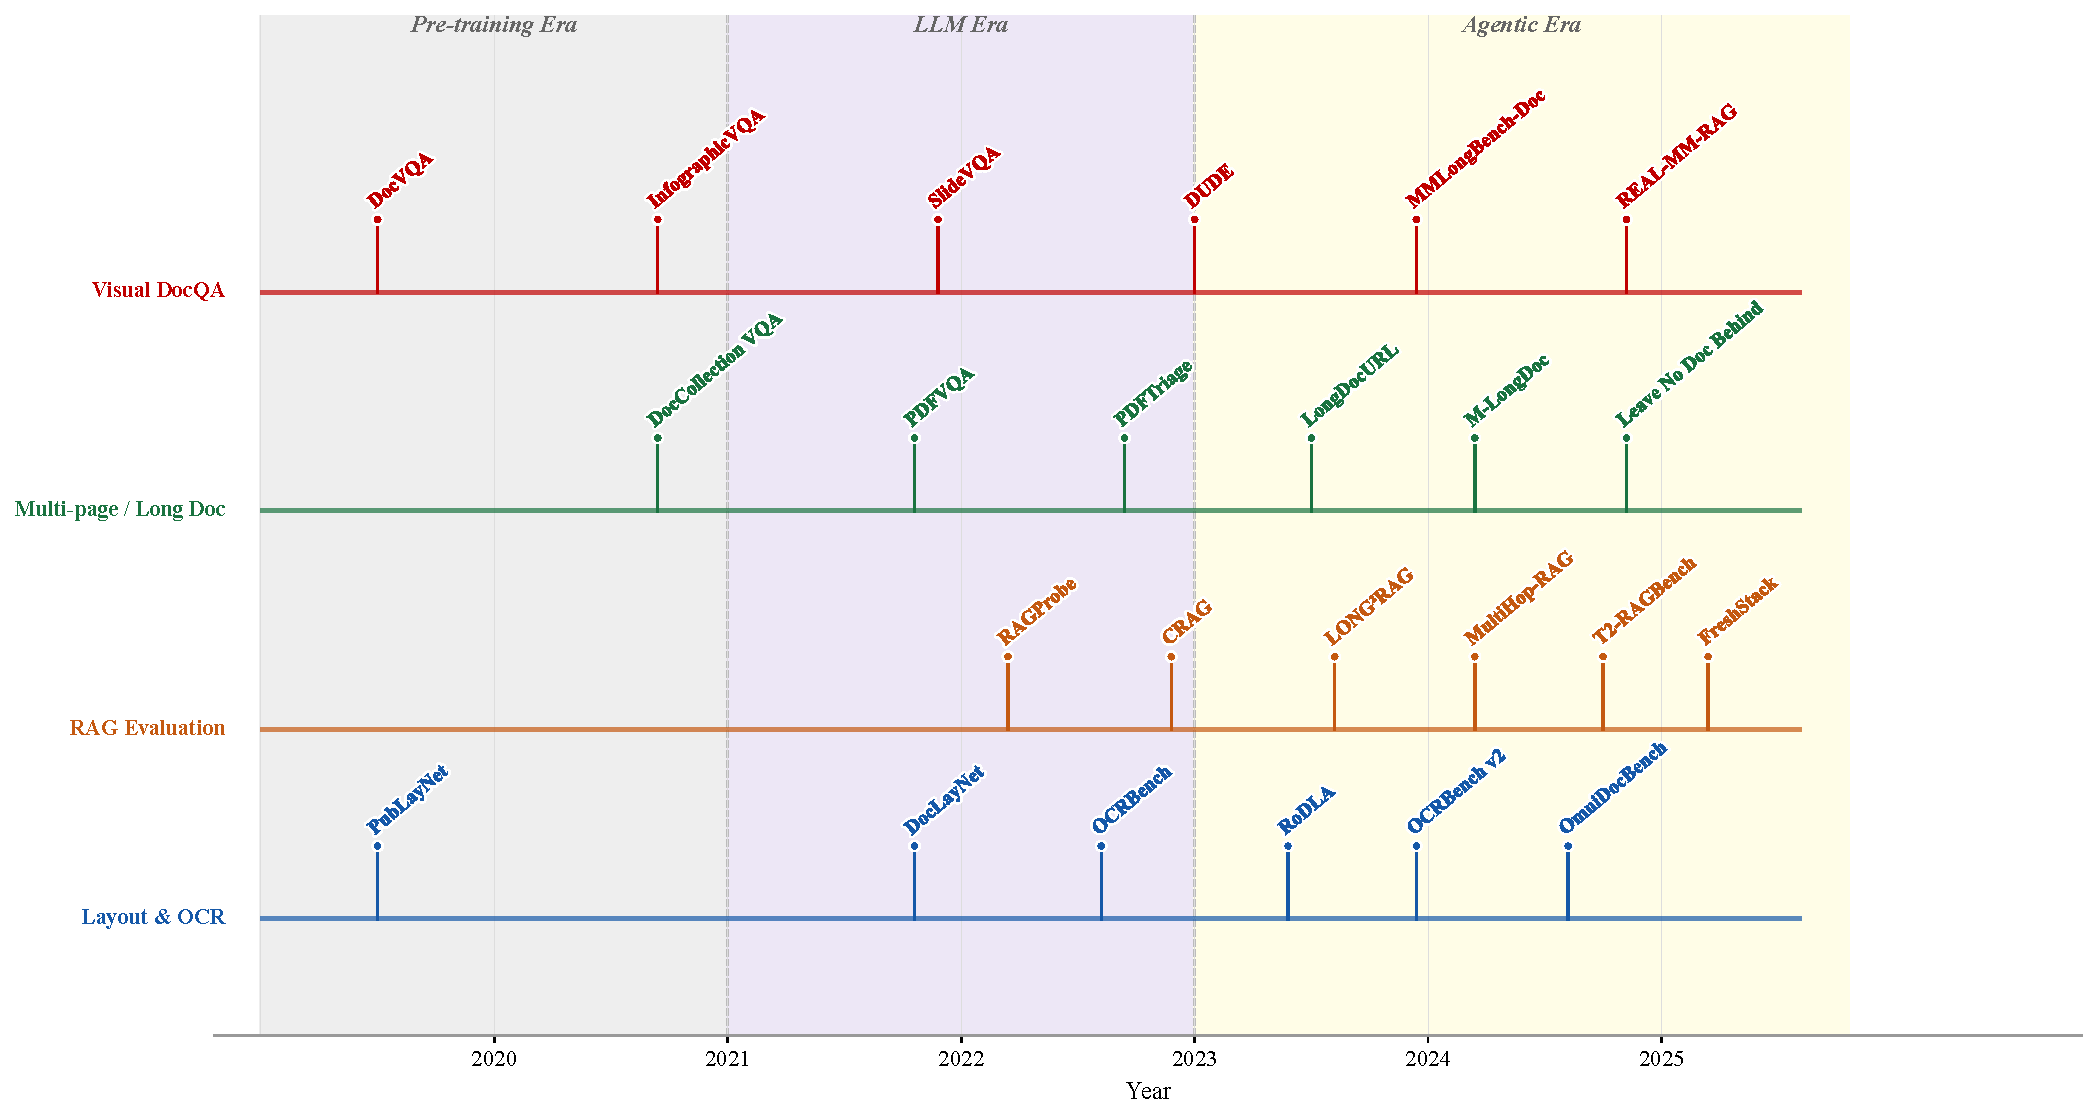
\includegraphics[
    width=0.95\textwidth,
    trim=0cm 0cm 0cm 0cm,
    clip
]{figs/fig10.pdf}
\caption{Benchmark landscape for document intelligence (2019--2025): evaluation datasets are organized into four categories---visual document question answering, multi-page and long-document understanding, retrieval-augmented generation evaluation, and layout analysis with optical character recognition---arranged chronologically by year of publication.}
\label{fig:benchmarks}
\end{figure*}

\subsection{Document QA and RAG Evaluation}

RAG-oriented evaluation explored complex question forms and systematic evaluation frameworks.

\subsubsection{General RAG Evaluation}

RAGProbe \cite{ragprobe2023} evaluated Retrieval-Augmented Generation covering complex question forms in real products (multiple sub-questions, cross-document, unanswerable). CRAG \cite{crag2024} designed task sets covering multiple domains, document structures, and question types for reproducible RAG architecture comparisons.

Explainable and controllable evaluation frameworks emerged. Unanswerability Evaluation for RAG \cite{unanswerablerag2024} measured whether systems correctly refuse unanswerable queries. LONG²RAG \cite{long2rag2024} systematically measured capabilities in ``reading long text, retrieving multiple documents, and generating long answers.'' Fact, Fetch, and Reason \cite{factfetchreason2024} measured end-to-end system performance with multi-hop QA requiring numerical calculation, table queries, and temporal reasoning.

\subsubsection{Domain-Specific and Multilingual Evaluation}

Chinese and domain-specific datasets expanded coverage. CRUD-RAG \cite{crudrag2024} was a large-scale Chinese benchmark abstracting four major application types from ``user interaction with knowledge bases.'' LegalBench-RAG \cite{legalbenchragr2024} measured precision retrieval on complex legal documents. OmniEval \cite{omnieval2024} automatically assessed financial RAG/Agent systems. RAGCare-QA \cite{ragcareqa2025} provided medical RAG evaluation for theoretical medical knowledge QA. RAGPPI \cite{ragppi2024} evaluated PPI-related biological question answering for drug target discovery.

\subsubsection{Long-Context and Multimodal Benchmarks}

Document and multimodal long-context benchmarks matured rapidly. M3DocVQA \cite{m3docvqa2024} provided open-domain, multi-page, multi-document DocVQA. MMLongBench-Doc \cite{mmlongbenchdoc2024} and MMDocBench \cite{mmdocbench2024} tested LVLMs in real long-document PDF scenarios. DOCBENCH \cite{docbench2024} assessed end-to-end document reading system capabilities. LongDocURL \cite{longdocurl2024} focused on complex PDFs of dozens or hundreds of pages, dividing tasks into Understanding, Reasoning, and Locating. M-Longdoc \cite{mlongdoc2024} evaluated ``multimodal ultra-long document understanding'' on hundreds of pages.

\subsection{Real-World Image-Text Interaction Document Evaluation}

Recent datasets involve image-text interaction for real-world settings.

\subsubsection{Multimodal RAG Evaluation}

REAL-MM-RAG \cite{realmmrag2025} focused on real enterprise/document scenarios, emphasizing ``difficult retrieval and high robustness'' across text, tables, and images. CRAG-MM \cite{cragmm2024} was a comprehensive RAG benchmark for multi-modal, multi-person multi-turn dialogue scenarios, focusing on ``wearable devices + visual QA + retrieval augmentation.'' Visual-RAG \cite{visualrag2025} provided text-to-image RAG benchmarks with visual knowledge-intensive questions.

Seeing Through the MiRAGE \cite{mirage2025} measured factuality and citation quality when retrieving, generating, and citing from multimodal sources. UNIDOC-BENCH \cite{unidocbench2025} extracted pages from real enterprise-level PDFs, annotating text blocks, tables, and images with evidence links. VisR-Bench \cite{visrbench2025} proposed a multi-lingual long-document visual retrieval benchmark focusing on ``retrieving the appropriate page from long multi-page documents and then answering.''

\subsubsection{Multi-Hop and Complex Reasoning}

Multi-hop retrieval and reasoning benchmarks developed. MultiHop-RAG \cite{multihoprag2024} systematically evaluated retrieval and reasoning in complex multi-hop QA. DocHop-QA \cite{dochopqa2025} focused on ``cross-document, multi-structure, multi-step reasoning'' scenarios constructed from scientific PDFs. FanOutQA \cite{fanoutqa2024} focused on ``fan-out'' questions requiring simultaneous information integration across numerous entities and documents. MHTS \cite{mhts2025} systematically controlled reasoning difficulty for finer RAG evaluation.

\subsubsection{Structured and Heterogeneous Data}

RAG evaluation on structured heterogeneous data received increasing attention. RAG over Tables \cite{ragovertables2025} provided benchmarks for multi-table QA on large-scale tabular corpora. T2-RAGBench \cite{t2ragbench2025} was a text-table hybrid RAG benchmark for the financial domain. mmRAG \cite{mmrag2025} provided a modular benchmark for heterogeneous/multimodal RAG systems across text, tables, and knowledge graphs.

Dynamic and temporal evaluation emerged. DRAGON \cite{dragon2024} was a dynamic RAG benchmark for news scenarios with continuously changing corpora. FreshStack \cite{freshstack2025} evaluated technical document retrieval in rapidly evolving technical fields.

\subsubsection{Long-Context and Retrieval-Free Control}

Long-context and retrieval-free control evaluations were proposed. LaRA \cite{lara2025} evaluated whether LLMs should rely on ultra-long context or external retrieval. Ko-LongRAG \cite{kolongrag2025} was a Korean long-context RAG benchmark using ``retrieval-free construction.'' Summary of a Haystack \cite{summaryhaystack2024} tested robust long-text understanding in million-token contexts. Are We on the Right Way for Assessing Document RAG? \cite{rightwaydocumentrag2025} analyzed deficiencies of current benchmarks and proposed Double-Bench as an alternative.

\subsubsection{Perceptual and Structural Foundations}

Visual document understanding datasets characterized real document complexity at visual, structural, and linguistic levels. RoDLA \cite{rodla2024} systematically evaluated layout detection stability under real interference. U-DIADS-Bib \cite{udiadsbib2024} focused on pixel-level semantic layout segmentation for ancient manuscripts. M6Doc \cite{m6doc2023} emphasized real scenarios, multiple formats, multiple languages, and complex layouts. MosaicDoc \cite{mosaicdoc2025} provided a large-scale Chinese-English bilingual benchmark from newspapers and magazines. HW-MLVQA \cite{hwmlvqa2025} and MTVQA \cite{mtvqa2025} evaluated multilingual handwritten and text-centric visual QA. IconQA \cite{iconqa2024} focused on diagram reasoning with abstract charts and textbook illustrations.
